\documentclass{jarticle}
\usepackage{mathtools, multicol}
\usepackage{color}
\usepackage{url}
\usepackage{comment}
\usepackage{here}
\usepackage{txfonts}
\usepackage{listings, jlisting}
\usepackage{latexsym}

\renewcommand{\lstlistingname}{リスト}

\lstdefinestyle{customplain}{
  belowcaptionskip=1\baselineskip,
  breaklines=true,
  frame=tRBl,
  xleftmargin=\parindent,
  language=,
  showstringspaces=false,
  numbers=left,
  basicstyle=\footnotesize\ttfamily,
  keywordstyle=\bfseries\color{black},
  commentstyle=\itshape\color{black},
  identifierstyle=\color{black},
  stringstyle=\color{black},
}

% 余白の設定
\usepackage[top=20truemm, bottom=16truemm, left=10truemm, right=10truemm]{geometry}

% 図の挿入
\usepackage[dvipdfm]{graphicx}

% より複雑な数学記号
\usepackage{amsmath,amssymb}

% 図の通し番号
\usepackage{subfigure}

\newcommand{\todayd}{%
\the\year.{\ifnum \month < 10 0\the\month \else \the\month \fi}.%
{\ifnum \day < 10 0\the\day \else \the\day \fi}}


\makeatletter

\def\@thesis{人工知能}
\def\id#1{\def\@id{#1}}
\def\department#1{\def\@department{#1}}

\def\@maketitle{
	\begin{center}
		{\huge \@thesis \par} %大きなタイトルが記載される部分
		\vspace{10mm}
		{\LARGE\bf \@title \par} % タイトル部分
		\vspace{20mm}
		{\Large 提出締切: 2013.11.07\par} % 提出年月日部分
		\vspace{5mm}
		{\Large 提出日:  \@date \par} % 提出年月日部分
		\vspace{20mm}
		{\Large \@department \par} % 所属部分
		\vspace{10mm}

		{\Large\@id } % 学籍番号部分
		{\Large \@author} % 氏名 
	\end{center}
\par\vskip 1.5em
}

\makeatother

\title{第2回講義課題 課題番号06}
\date{\todayd}
\department{工学部電子情報工学科}
\id{03-123006}
\author{岩成達哉}


\begin{document}

\begin{titlepage}
	\setlength{\topmargin}{1.1in}
	\vspace{100mm}
	\maketitle
\end{titlepage}


\section{ATMSを用いたN-Queens問題の解答プログラム}
今回は,ATMSを用いる例として,N-Queens問題を解き,解法の数を出力するプログラムを作成した.プログラムは,参考URL\cite{ref:atms}\cite{ref:nqueen}を基にCommon Lispによって記述した.その実行結果をリスト\ref{code:output}に示した.これは対称な解も含めて出力している.プログラムは,atms.lispとnqueens.lispの2種類である.

\lstset{style=customplain}
\lstinputlisting[caption=実行結果,label=code:output]{../output.txt}



% ---
\section{ATMSによるN-Queensの解法説明}
% ---
\subsection{ATMSの主要な動作}

ATMSは,Assumption-based TMSの略であり,仮説を基にして,推論を繰り返し,矛盾のない仮説集合(環境)を求めることが狙いである.ここで用語をいくつか取り上げると,「仮説」は成立するかどうかわからないもの,「前提」はいつも整理するもの,「ノード」は推論結果や仮説,前提のいずれか,「正当化」は推論結果が成立する理由付けを行うことである.また,ATMSでは,矛盾する条件を「Nogood」と呼び,推論に用いる.JTMSと違い,ATMSは導出と仮説ノードを分ける\cite{ref:atms_basic}.ATMSでは,ノードに対して「ラベル」を付与する.ラベルは複数の「環境」から成り,環境は複数の「仮説」から成る\cite{ref:atms_label}.これは例えば,図\ref{fig:label}のようになる\cite{ref:atms_label}.

\begin{figure}[H]
	\begin{center}
	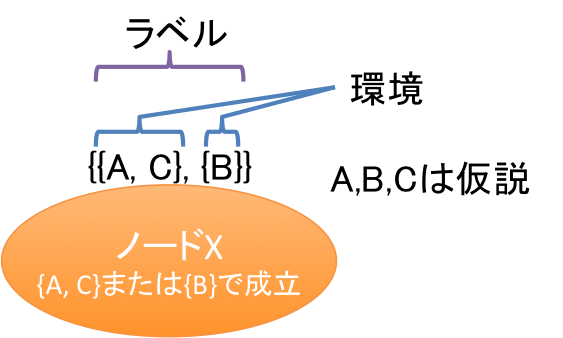
\includegraphics[width=80mm]{image/label.png}
	\caption{ラベル,環境,仮説,ノードの整理}
	\label{fig:label}
	\end{center}
\end{figure}

このノードと,仮説に基づいて,矛盾のない仮説の集合を求めるわけである.ATMSでは,バックトラックを行わず,仮説とNogoodを用意しておくことで,仮説の検証を全ての場合について行うことができる.今回のN-Queensの問題では,このラベルを更新することで解の個数を求めるということを行った.ラベルの更新は例えば,図\ref{fig:update_label}のようになる.ノードXのラベルとノードYのラベルの全ての組み合わせを列挙する.この際に,環境が他のより強い条件に含まれるならばそれを除く.このような操作で,ノードZのラベルとしては,$\{A, B, C\}$が除かれて,3つの環境が残る.また,Nogoodとなるような環境が含まれた場合はそれも除く.例えば,$\{B, D\}$がNogoodであるならば,ノードZのラベルは,$\{\{A, C\},\{C, D\}\}$となる.

\begin{figure}[H]
	\begin{center}
	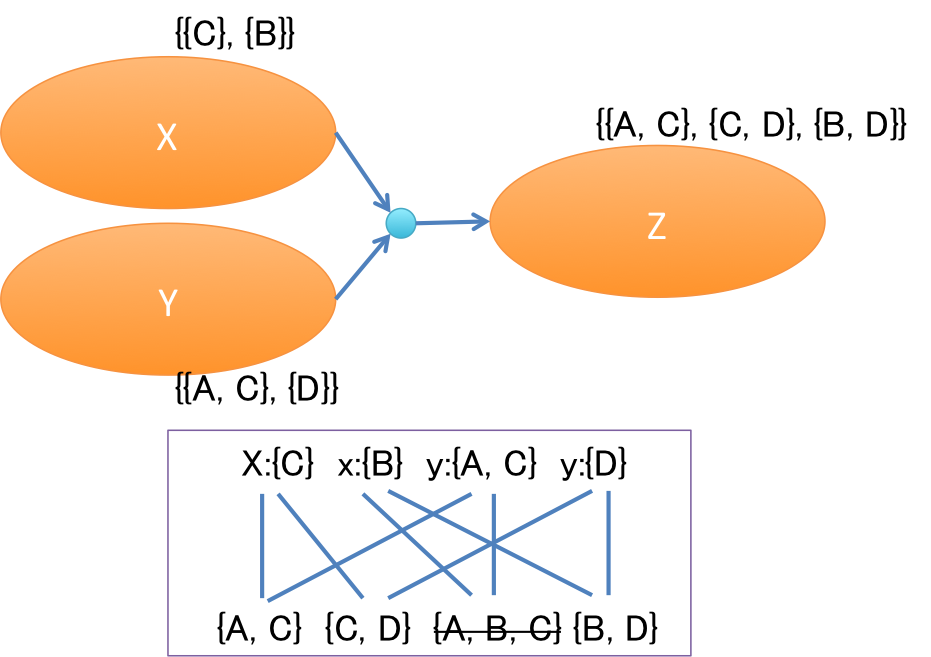
\includegraphics[width=100mm]{image/update_label.png}
	\caption{ラベルの更新}
	\label{fig:update_label}
	\end{center}
\end{figure}





% ---
\subsection{仮説とNogoodの作成}

さて,以上がATMSの主要な動作であるが,この仕組をN-Queenに適用する.これまでの内容からわかるように,ATMSでは仮説とNogoodを列挙することから始める.N-Queensでは,N個のQueenを$N*N$の盤上で,縦・横・斜めの列に一つずつしかないように配置する.例えば,8-Queensでは,図\ref{fig:a_sol}が解の1つである.

\begin{figure}[H]
	\begin{center}
	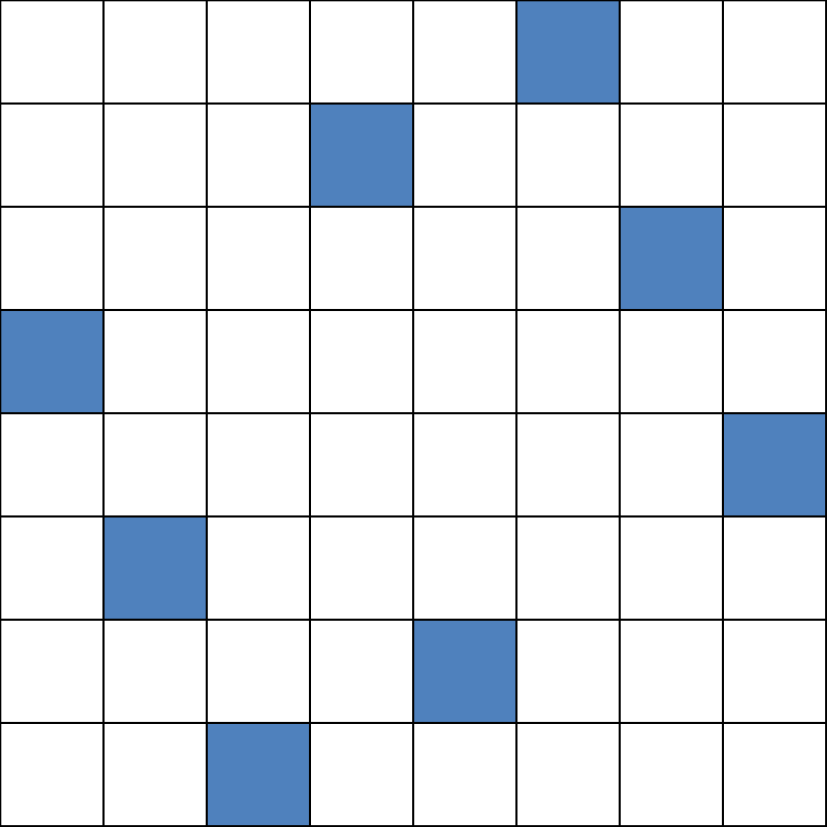
\includegraphics[width=60mm]{image/a_sol.png}
	\caption{8クイーンの1つの解}
	\label{fig:a_sol}
	\end{center}
\end{figure}

仮説を作る際には,$N*N$の位置にQueenが設置される可能性があるため,単純に$N*N$の数だけその位置についての仮説を用意する.次に,Nogoodを作成するわけだが,N-Queenの解答では「同じ列には1つのQueenしか配置されない」ことを利用する.つまり,同じ列にQueenが配置されることを考えずに,
\begin{enumerate}
	\item 同じ行にQueenがいないか
	\item 斜めの列にQueenがいないか
\end{enumerate}
の2つを考えればよいとする.すると,検証を大きく減らすことができる.したがって,Nogoodの作成には,2つのQueenの位置を$(i_1, j_1),(i_2, j_2)$とすると,
\begin{enumerate}
	\item $j$については考えず,$i$が同じか
	\item $|i_1 - i_2| = |j_1 - j_2|$か
\end{enumerate}
を確認し,どちらか一方でも成り立てば,その2つのQueenの位置を記憶するのである.さて,以上で仮説とNogoodを作成することができた.次は,これらを用いてノードを作り,ラベルを更新していく.





%---
\subsection{ノードの作成とラベルの更新,解の導出}
まずは,1列目にQueenを置く仮説$(k,1) (k = 1..N)$全てに対してノードを作り,それらを正当化する.なぜなら,最初のQueenの位置は任意であり,この時点では矛盾を含んでいないからである.これは,図\ref{fig:first-position}のようになる.

\begin{figure}[H]
	\begin{center}
	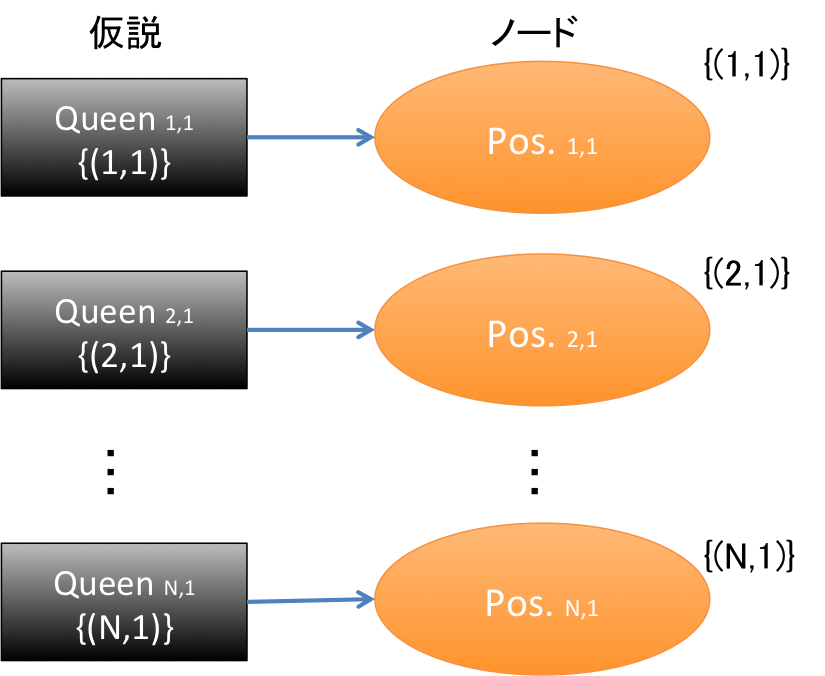
\includegraphics[width=80mm]{image/first-position.png}
	\caption{最初の列}
	\label{fig:first-position}
	\end{center}
\end{figure}

次は,2列目に移行し,それぞれのノードと,2列目にQueenを置く仮説を用いて,ラベルを更新する.このときに,Nogoodとなる環境を含むノードがあれば,そのノードは正当化できない.この様子を,図\ref{fig:repetition}に示した.上部の$\{(1,1),(1,2)\}$はNogoodに含まれているので,正当化されず,$\{(1,1),(3,2)\}$は正当化される.この操作によって,残ったノードのみについて,$N$列目まで同様の操作を繰り返していく.

そして,最後まで残ったノードを数え上げれば,それが解法の数になるというアルゴリズムである.

\begin{figure}[H]
	\begin{center}
	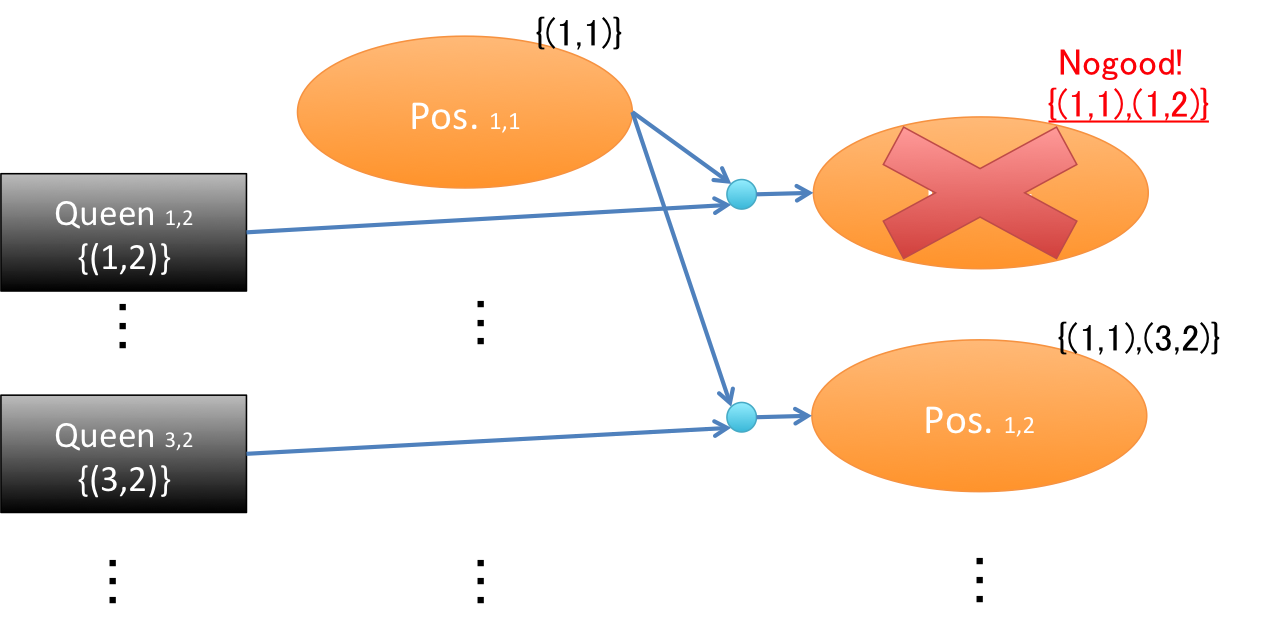
\includegraphics[width=140mm]{image/repetition.png}
	\caption{ラベルの更新}
	\label{fig:repetition}
	\end{center}
\end{figure}





%---
\section{ATMSの覆面算への利用と解法の考察}
さて,ここまでは,N-Queenに対してATMSを利用する方法について見てきた.次は,このアルゴリズムを覆面算へ適用して,解法を考察する.

まずは,仮説とNogoodを作る.覆面算は,最大10個の文字に,$0〜9$の数字を当てはめて,正しい式を導くことが目的である.例えば,

\begin{center}
{\Large{
$
\begin{array}{rr}
  &  BASE\\
+ &  BALL \\ \hline
     & GAMES
\end{array}
$
}} \\
\end{center}

のような数式が考えられ,同じ文字には同じ数字が入る.仮説としては,単純にそれぞれの文字に$0〜9$の数字が入ること,つまり$9^n(nは文字の種類)$個を用意する.Nogoodとしては,
\begin{enumerate}
	\item 違う文字に同じ数字が入る
	\item 同じ桁の数値を足して(mod 10)をとったものが,同じ桁の答えの数値でも$数値-1$でもない
\end{enumerate}
を考える.

これによって,ラベルを更新していき,全ての文字に数値が対応したところで,足される数値2つの和と答えの数値が一致するものを数え上げれば解の数が求まる.

この方法によって,ATMSを利用して覆面算は解くことができると考えられるが,実装には至らなかった.

\begin{thebibliography}{n}
\bibitem{ref:atms}
『人工知能特論』(last accessed at 2013/11/07),\url{http://winnie.kuis.kyoto-u.ac.jp/~okuno/Lecture/02/AI/ai-02-9-ohp.pdf}

\bibitem{ref:nqueen}
『Peter@Norvig.com』(last accessed at 2013/11/07),\url{http://norvig.com/ltd/test/atms.lisp}

\bibitem{ref:atms_basic}
Takeuchi Lab:『講義資料置き場>知識工学』(last accessed at 2013/11/07),\url{http://cl.it.okayama-u.ac.jp/kougi/data/knowledge}

\bibitem{ref:atms_label}
情報工学教育類/産業戦略工学専攻 伊藤孝行:『知能処理アルゴリズム論 第6回 推論システムとTMS』(last accessed at 2013/11/07),\url{http://www.itolab.nitech.ac.jp/~ito/Lecture/IntelligentAlgorithm2011/IntelligentAlgorithm6.pdf}

\bibitem{ref:ai_book}
伊庭斉志:『人工知能と人工生命の基礎』,オーム社,pp.37-51,(平成25年5月24日)

\end{thebibliography}

\end{document}












